
\section{Introduction}
\subsection{Introduction}
\begin{frame}{Introduction}
Nous présenterons l'article\\
\alert{\textit{Tiny Web Serices: Design and Implementation of Interoperable and Evolvable Sensor Networks}}\\
Dont les travaux et la rédaction ont été réalisés par\\
Nissanka B. \textsc{Priyantha}, Aman \textsc{Kansal}, Mishel \textsc{Goraczko} et Feng \textsc{Zhao} pour Microsoft Research.
\begin{itemize}
\item Objet de la recherche : proposer une solution pour un réseau de capteurs basé sur les web services. 
\item Idée : si différents capteurs utilisent une couche applicative commune et bien connue, alors ils peuvent faire partie d'un réseau évolutif accessible à différentes applications. Pour chaque nouvelle application on peut réutiliser les capteurs dont on dispose déjà pour atteindre l'objectif de l'application.
\end{itemize}
Toutes les figures proviennent de cet article.
\end{frame}

\begin{frame}{Exemple}
Les auteurs illustrent ce point en prenant comme exemple une application de gestion de l'énergie basée sur les capteurs pour la sécurité et pour le système d'alerte médicale. 
\begin{figure}
  \centering
  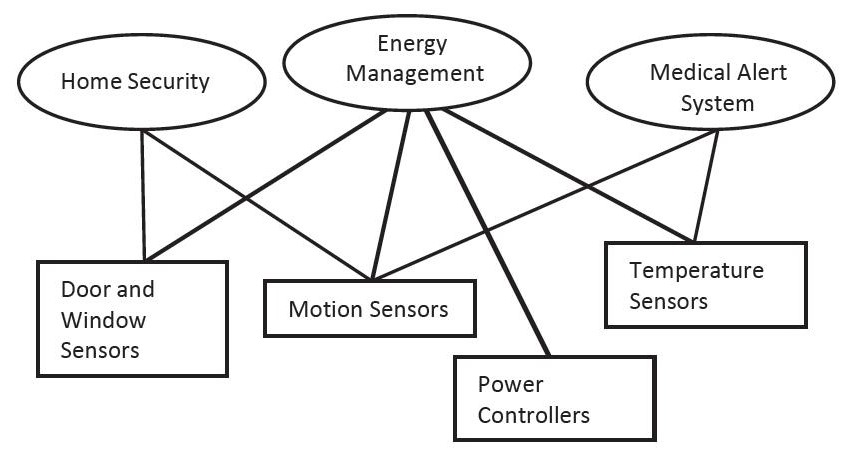
\includegraphics[scale=0.4]{figures/exemple.jpg}
  \caption{Exemple de réseau}
 \end{figure} 
\end{frame}


\begin{frame}
Pour réaliser cela, nous avons besoin de 2 fonctionnalités :
\begin{itemize}
\item Données structurées : compréhension des applications (exemple XML)
\item Accès aux fonctionnalités par appel de fonction : description des fonctionnalités du capteur accessibles par programmation
\end{itemize}
Ces fonctionnalités existent déjà pour se connecter à Internet par exemple et sont disponibles au travers des web services.\\ Le challenge dans cette approche consiste à minimiser le coût en ressources pour supporter ces services. Ce coût n'est pas négligeable pour les capteurs sans fil de faible puissance qui doivent fonctionner sur batterie pendant des années.
\end{frame}

\begin{frame}
But : 
\begin{itemize}
\item estimer le coût en ressources
\item identifier les choix de design qui minimisent ce coût
\item analyser l'impact de ces choix sur la généralité de l'interface
\end{itemize}

\end{frame}

\begin{frame}{Capteur utilisé}
Capteur prototype utilisant :
\begin{itemize}
\item un processeur MSP430 tournant à 6Mhz, contenant 48k de ROM et ayant une consommation énergétique équivalente à celle de la plupart des capteurs de faible puissance.
\item une interface radio IEEE 802.15.4 dont la vitesse maximale de transfert est de 250kbps.
\end{itemize}
\begin{figure}
  \centering
  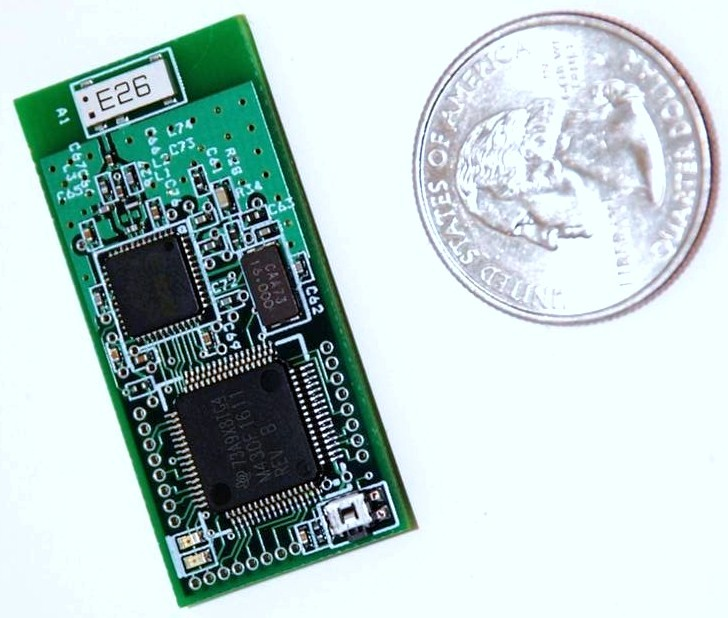
\includegraphics[scale=0.15]{figures/tws08-000.jpg}
  \caption{Capteur sans fil utilisé pour les expérimentations}
 \end{figure} 
\end{frame}

\section{Travaux liés}
\begin{frame}{Travaux liés}
Différents travaux ont été consultés pour réaliser cette étude :
\begin{itemize}
\item XML sur des capteurs : format standard de données
\item Services web embarqués 
\item Implémentation de web services : Devices Profile for Web Services (DPWS), utilisation de passerelles.
\item Couche réseau : nécessaire pour supporter la couche applicative
\item WS-Eventing : support du sleep mode et duty cycle
\item XML compression : gain de mémoire
\end{itemize}
La différence majeure entre ces travaux et cette étude est la contrainte en ressources des appareils considérés.
\end{frame}
\section{Web services}
\begin{frame}{Présentation des web services}
Ils fournissent un mécanisme pour permettre à des applications d’utiliser des ressources à distance de la même façon que des ressources locales.
Les standards définissent 2 composants clés:
\begin{itemize}
\item Ports : appel aux méthodes disponibles sur le serveur  
\item Bindings : protocoles réseaux supportés
\end{itemize}
Ces 2 composants sont définis via le Web Services Description Language (WSDL), les spécifications du web service est référencé par sa description WSDL.
\end{frame}

\begin{frame}{Avantages}
\begin{itemize}
\item Partage des ressources de manière très flexible : meilleure performance des applications existantes, déploiement de nouvelles applications sans forcément de nouveaux capteurs.
\item Plus facile à programmer : la description WSDL peut facilement être traduite en un langage haut niveau et le programmeur voit uniquement un objet avec les méthodes appropriées.
\item Facilité d’intégration dans les réseaux d’entreprise à travers Internet : il existe déjà beaucoup d’applications réseau basées sur les web services. Si les capteurs disposent d’interfaces similaires, alors les données physiques générées peuvent être utilisées pour donner de nouvelles possibilités aux applications existantes.
\item Suppression des gateways (passerelles) : la traduction des formats de messages  custom  de chaque fabricant n’est plus nécessaire.
\end{itemize}
\end{frame}
\begin{frame}
En plus de tous ces avantages liés à la couche applicative, le fait d’utiliser l’IP pour la couche réseau présente aussi des avantages : \begin{itemize}
\item facilité de gestion de réseau
\item utilisation de DHCP pour l’allocation d’adresses
\item valide pour différentes couches physiques
\end{itemize}

L’approche web-service est pensée pour améliorer l’interface entre les nœuds capteurs et les applications pour les utilisateurs finaux (end user). La programmation des nœuds n’est pas significativement affectée. Le seul impact est l’ajout de la description WSDL.

\end{frame}
\begin{frame}{Inconvénient}
Coût en ressource : à la base on crée des protocoles dédié afin d’optimiser les formats de message jusqu’au dernier bit pour réduire le coût en énergie des overheads dans les communications pour matcher les contraintes de ressources des réseaux de capteurs.
\\La question évidente vient alors : est-ce que les avantages offerts par les web services sont suffisamment important en comparaison du coût en ressources ou est-ce que le coût en ressource dû à l’utilisation d’une interaction basée sur les web services est acceptable ?

\end{frame}
